\documentclass[14pt]{extbook}
\usepackage{multicol, enumerate, enumitem, hyperref, color, soul, setspace, parskip, fancyhdr} %General Packages
\usepackage{amssymb, amsthm, amsmath, latexsym, units, mathtools} %Math Packages
\everymath{\displaystyle} %All math in Display Style
% Packages with additional options
\usepackage[headsep=0.5cm,headheight=12pt, left=1 in,right= 1 in,top= 1 in,bottom= 1 in]{geometry}
\usepackage[usenames,dvipsnames]{xcolor}
\usepackage{dashrule}  % Package to use the command below to create lines between items
\newcommand{\litem}[1]{\item#1\hspace*{-1cm}\rule{\textwidth}{0.4pt}}
\pagestyle{fancy}
\lhead{Progress Quiz 6}
\chead{}
\rhead{Version C}
\lfoot{1430-1829}
\cfoot{}
\rfoot{test}
\begin{document}

\begin{enumerate}
\litem{
Construct the lowest-degree polynomial given the zeros below. Then, choose the intervals that contain the coefficients of the polynomial in the form $x^3+bx^2+cx+d$.\[ -3 + 2 i \text{ and } -3 \]\begin{enumerate}[label=\Alph*.]
\item \( b \in [-5, 4], c \in [5.6, 7.3], \text{ and } d \in [0, 15] \)
\item \( b \in [7, 14], c \in [30.7, 35.8], \text{ and } d \in [32, 45] \)
\item \( b \in [-10, -6], c \in [30.7, 35.8], \text{ and } d \in [-46, -38] \)
\item \( b \in [-5, 4], c \in [-1.3, 3.2], \text{ and } d \in [-6, -3] \)
\item \( \text{None of the above.} \)

\end{enumerate} }
\litem{
Describe the end behavior of the polynomial below.\[ f(x) = -9(x + 3)^{2}(x - 3)^{3}(x + 7)^{5}(x - 7)^{5} \]\begin{enumerate}[label=\Alph*.]
\begin{multicols}{2}\item 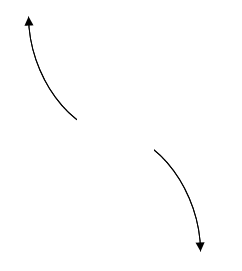
\includegraphics[width = 0.3\textwidth]{../Figures/polyEndBehaviorCopyAC.png}\item 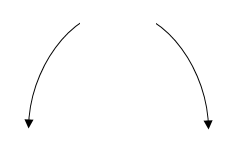
\includegraphics[width = 0.3\textwidth]{../Figures/polyEndBehaviorCopyBC.png}\item 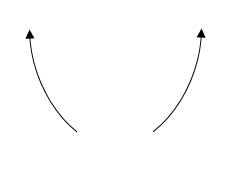
\includegraphics[width = 0.3\textwidth]{../Figures/polyEndBehaviorCopyCC.png}\item 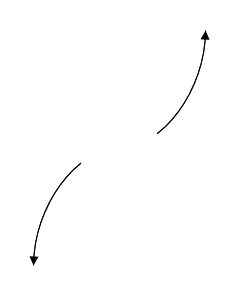
\includegraphics[width = 0.3\textwidth]{../Figures/polyEndBehaviorCopyDC.png}\end{multicols}\item None of the above.
\end{enumerate} }
\litem{
Describe the zero behavior of the zero $x = 7$ of the polynomial below.\[ f(x) = -6(x - 4)^{7}(x + 4)^{4}(x + 7)^{7}(x - 7)^{2} \]\begin{enumerate}[label=\Alph*.]
\begin{multicols}{2}\item 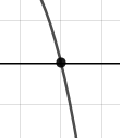
\includegraphics[width = 0.3\textwidth]{../Figures/polyZeroBehaviorAC.png}\item 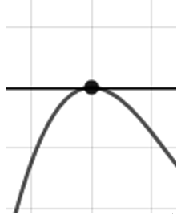
\includegraphics[width = 0.3\textwidth]{../Figures/polyZeroBehaviorBC.png}\item 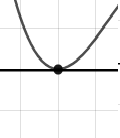
\includegraphics[width = 0.3\textwidth]{../Figures/polyZeroBehaviorCC.png}\item 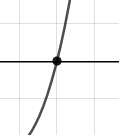
\includegraphics[width = 0.3\textwidth]{../Figures/polyZeroBehaviorDC.png}\end{multicols}\item None of the above.
\end{enumerate} }
\litem{
Construct the lowest-degree polynomial given the zeros below. Then, choose the intervals that contain the coefficients of the polynomial in the form $ax^3+bx^2+cx+d$.\[ \frac{5}{4}, -5, \text{ and } \frac{-4}{5} \]\begin{enumerate}[label=\Alph*.]
\item \( a \in [17, 27], b \in [86, 92], c \in [-71, -61], \text{ and } d \in [-100, -98] \)
\item \( a \in [17, 27], b \in [-59, -53], c \in [-192, -178], \text{ and } d \in [-100, -98] \)
\item \( a \in [17, 27], b \in [86, 92], c \in [-71, -61], \text{ and } d \in [98, 103] \)
\item \( a \in [17, 27], b \in [140, 144], c \in [220, 226], \text{ and } d \in [98, 103] \)
\item \( a \in [17, 27], b \in [-98, -90], c \in [-71, -61], \text{ and } d \in [98, 103] \)

\end{enumerate} }
\litem{
Construct the lowest-degree polynomial given the zeros below. Then, choose the intervals that contain the coefficients of the polynomial in the form $ax^3+bx^2+cx+d$.\[ \frac{3}{4}, \frac{1}{2}, \text{ and } 6 \]\begin{enumerate}[label=\Alph*.]
\item \( a \in [8, 11], b \in [-65, -57], c \in [61, 72], \text{ and } d \in [-19, -16] \)
\item \( a \in [8, 11], b \in [-40, -35], c \in [-61, -55], \text{ and } d \in [-19, -16] \)
\item \( a \in [8, 11], b \in [51, 60], c \in [61, 72], \text{ and } d \in [17, 19] \)
\item \( a \in [8, 11], b \in [-65, -57], c \in [61, 72], \text{ and } d \in [17, 19] \)
\item \( a \in [8, 11], b \in [-48, -40], c \in [-17, -9], \text{ and } d \in [17, 19] \)

\end{enumerate} }
\litem{
Which of the following equations \textit{could} be of the graph presented below?
\begin{center}
    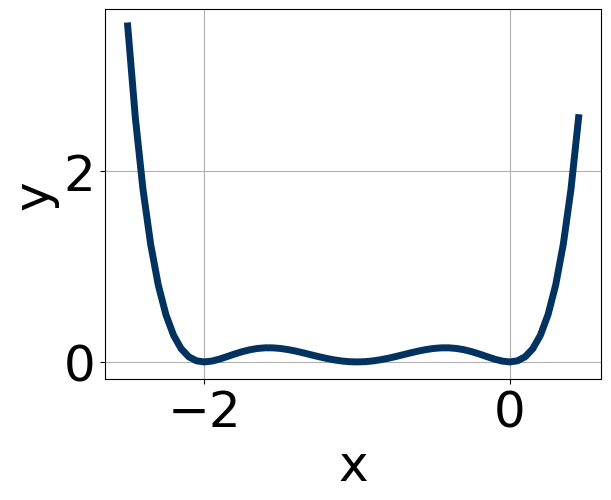
\includegraphics[width=0.5\textwidth]{../Figures/polyGraphToFunctionCopyC.png}
\end{center}
\begin{enumerate}[label=\Alph*.]
\item \( -13(x - 2)^{10} (x - 1)^{9} (x + 1)^{7} \)
\item \( -5(x - 2)^{11} (x - 1)^{10} (x + 1)^{5} \)
\item \( 3(x - 2)^{8} (x - 1)^{7} (x + 1)^{10} \)
\item \( -10(x - 2)^{6} (x - 1)^{6} (x + 1)^{9} \)
\item \( 6(x - 2)^{10} (x - 1)^{7} (x + 1)^{9} \)

\end{enumerate} }
\litem{
Which of the following equations \textit{could} be of the graph presented below?
\begin{center}
    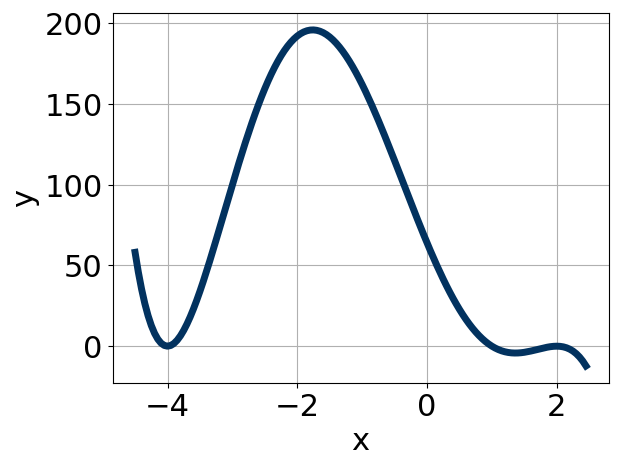
\includegraphics[width=0.5\textwidth]{../Figures/polyGraphToFunctionC.png}
\end{center}
\begin{enumerate}[label=\Alph*.]
\item \( -15(x + 3)^{8} (x + 4)^{5} (x - 1)^{9} \)
\item \( 11(x + 3)^{10} (x + 4)^{6} (x - 1)^{9} \)
\item \( -11(x + 3)^{6} (x + 4)^{4} (x - 1)^{11} \)
\item \( 16(x + 3)^{4} (x + 4)^{8} (x - 1)^{4} \)
\item \( -17(x + 3)^{4} (x + 4)^{6} (x - 1)^{10} \)

\end{enumerate} }
\litem{
Describe the zero behavior of the zero $x = 4$ of the polynomial below.\[ f(x) = -2(x - 3)^{4}(x + 3)^{2}(x - 4)^{9}(x + 4)^{8} \]\begin{enumerate}[label=\Alph*.]
\begin{multicols}{2}\item 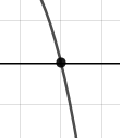
\includegraphics[width = 0.3\textwidth]{../Figures/polyZeroBehaviorCopyAC.png}\item 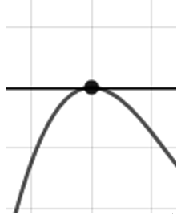
\includegraphics[width = 0.3\textwidth]{../Figures/polyZeroBehaviorCopyBC.png}\item 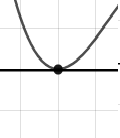
\includegraphics[width = 0.3\textwidth]{../Figures/polyZeroBehaviorCopyCC.png}\item 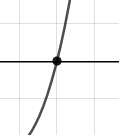
\includegraphics[width = 0.3\textwidth]{../Figures/polyZeroBehaviorCopyDC.png}\end{multicols}\item None of the above.
\end{enumerate} }
\litem{
Construct the lowest-degree polynomial given the zeros below. Then, choose the intervals that contain the coefficients of the polynomial in the form $x^3+bx^2+cx+d$.\[ -5 - 3 i \text{ and } 3 \]\begin{enumerate}[label=\Alph*.]
\item \( b \in [6, 12], c \in [3.05, 4.75], \text{ and } d \in [-104, -101] \)
\item \( b \in [-11, -5], c \in [3.05, 4.75], \text{ and } d \in [101, 108] \)
\item \( b \in [-6, 4], c \in [-0.86, 0.21], \text{ and } d \in [-14, -3] \)
\item \( b \in [-6, 4], c \in [1.77, 2.48], \text{ and } d \in [-17, -13] \)
\item \( \text{None of the above.} \)

\end{enumerate} }
\litem{
Describe the end behavior of the polynomial below.\[ f(x) = -5(x - 6)^{3}(x + 6)^{6}(x + 4)^{4}(x - 4)^{6} \]\begin{enumerate}[label=\Alph*.]
\begin{multicols}{2}\item 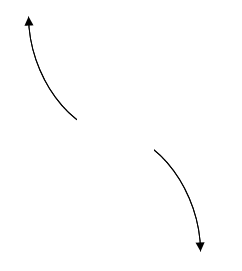
\includegraphics[width = 0.3\textwidth]{../Figures/polyEndBehaviorAC.png}\item 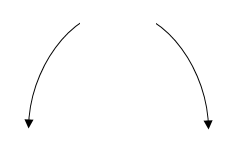
\includegraphics[width = 0.3\textwidth]{../Figures/polyEndBehaviorBC.png}\item 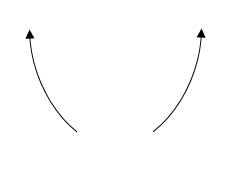
\includegraphics[width = 0.3\textwidth]{../Figures/polyEndBehaviorCC.png}\item 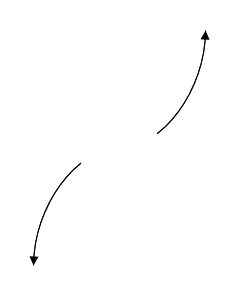
\includegraphics[width = 0.3\textwidth]{../Figures/polyEndBehaviorDC.png}\end{multicols}\item None of the above.
\end{enumerate} }
\end{enumerate}

\end{document}